\providecommand{\main}{..}
\documentclass[\main/main.tex]{subfiles}
\begin{document}
\chapter{Technologies}
\section{Cluster computing}
Modern applications require to deal with immense amount of data as quick as possible. In many of these applications, data is extremely regular, so there is opportunity to exploit parallelism. Examples of possible applications are:
\begin{itemize}
    \item Web page ranking
    \item Social networks analysis
    \item Parallelizable computations
\end{itemize}
This parallelization is not achieved using a super computer that can handle the computation, but is achieved using "computing clusters". Computing clusters are large collections of commodity hardware, including conventional processors, connected by Ethernet network. The software stack begins with a new form of file system, called a “distributed file system,” which features much larger units than the disk blocks in a conventional operating system. Distributed file systems also provide replication of data or redundancy to protect against the frequent media failures that occur when data is distributed over thousands of low-cost compute nodes. \cite{leskovec_rajaraman_ullman_2020}

\subsection{Big data}
Big data is high-volume, high-velocity and/or high-variety information assets that demand cost-effective, innovative forms of information processing that enable enhanced insight, decision making, and process automation.\cite{bigdatagartner}
\begin{itemize}
    \item \textbf{Volume}: the magnitude of data. Big data sizes could be terabytes or even petabytes
    \item \textbf{Variety}: the structural heterogeneity in a dataset. Data could be structured, semi-structured or unstructured.
    \item \textbf{Velocity}: data generation rate. Data analysis speed is a strongly connected concept: higher the velocity, higher the needed analysis speed.
\end{itemize}
Other mentioned dimensions:
\begin{itemize}
    \item \textbf{Veracity}: the unreliability of some data sources. For example, social media sentiments are a uncertain data source, because they imply human judgement
    \item \textbf{Variability}: the variation in data flow rates
    \item \textbf{Complexity}: the heterogeneity of data sources. Being generated through a myriad of sources, big data must be cleaned and connected in order to be used
    \item \textbf{Value}: the importance of big data. Being characterized by a "low value density", a big quantity must be analyzed in order to obtain an high value
\end{itemize}\cite{Gandomi2015BeyondTH}
\subsection{Distributed file system}
To exploit cluster computing, data must be organized differently from the conventional file systems of single computers. This new organization is called Distributed file system (DFS) and is used as follows:
\begin{itemize}
    \item Files can be huge, possibly terabyte in size
    \item Files are rarely updated. They are read as input for calculation and possibly additional data is appended to files
\end{itemize}
Files are divided into chunks. Chunks are replicated on different computer nodes. If chunks are replicated on different racks so that a rack fail won't cause any data loss.
Examples of DFS are:
\begin{itemize}
    \item Google File System (GFS), the original of the class
    \item Hadoop Distributed File System (HDFS), an open-source DFS used with Hadoop
    \item Colossus, an improved version of GFS
\end{itemize}
\begin{figure}[h]
    \centering
    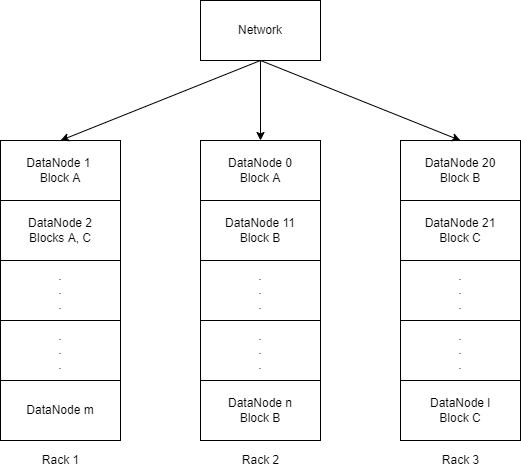
\includegraphics[scale=0.35]{images/cluster_computing/racks_dfs.png}
    \caption{DFS rack architecture}
    \label{fig:racks_dfs}
\end{figure}
\textbf{Rack failure}: If any problem causes the rack to not be able to intercommunicate with other racks.
\begin{figure}[h]
    \centering
    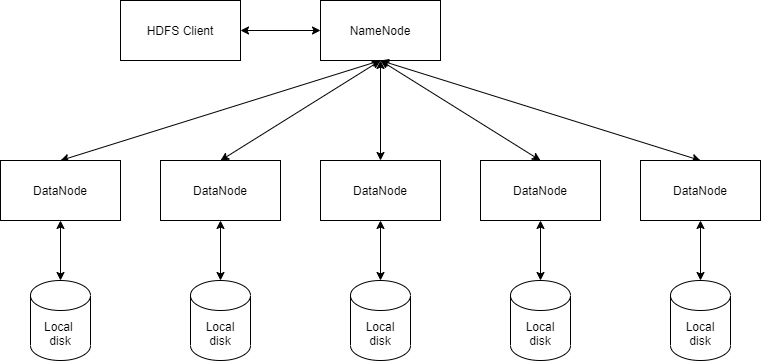
\includegraphics[scale=0.35]{images/cluster_computing/hdfs_architecture.png}
    \caption{HDFS  architecture}
    \label{fig:hdfs_architecture}
\end{figure}
\subsection{MapReduce}
MapReduce is a style of computing that is used to manage many large-scale, parallel computations in a way that is tolerant of hardware faults. A MapReduce computation consists of:
\begin{itemize}
    \item Map tasks: takes in input one or more data chunks and returns a sequence of \textit{key-value} pairs
    \item Reduce tasks: combine all the values associated with a key, one key at a time
\end{itemize}
\begin{figure}[h]
    \centering
    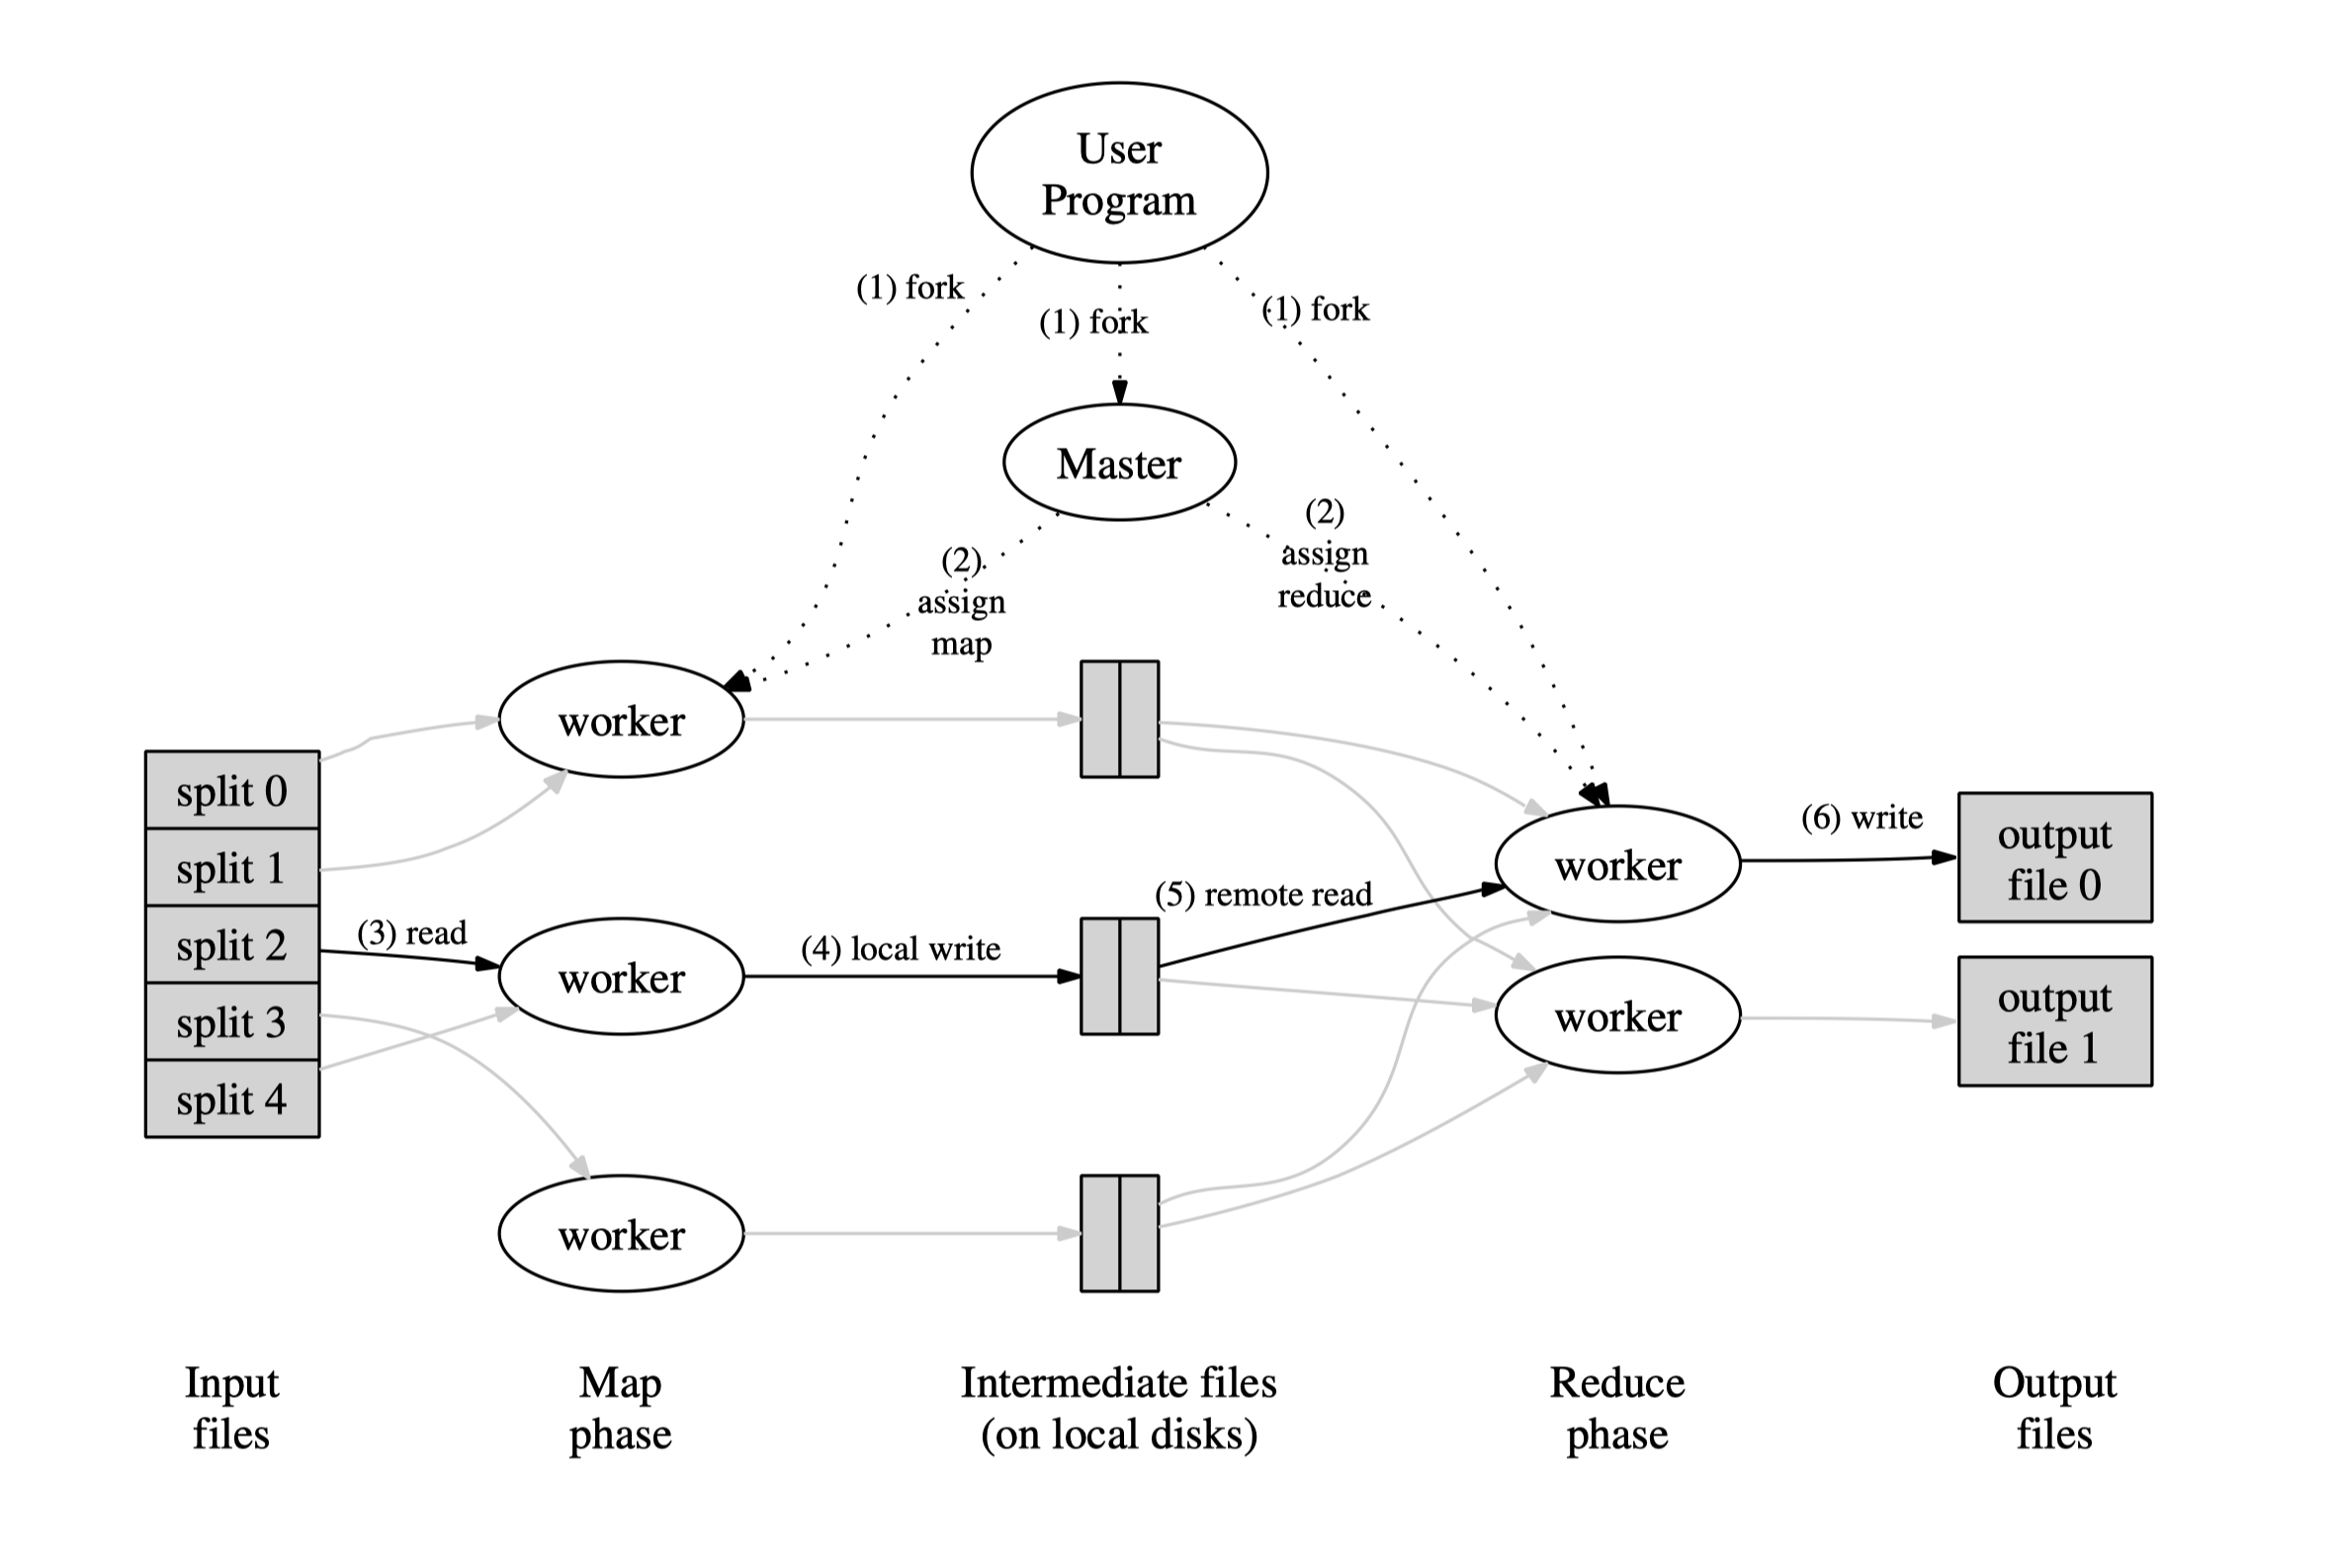
\includegraphics[scale=0.35]{images/cluster_computing/map_reduce_schema.png}
    \caption{MapReduce}
    \label{fig:map_reduce}
\end{figure}
An example of computation is visible in Figure \ref{fig:map_reduce}
\subsubsection{Map task}
The input files for a Map task are elements of any type: tuple, document, \dots //
A chunk is a collection of elements, and no element is stored across two chunks. 
A Map task produces zero or more key-value pairs, with keys not necessarily uniques.
\subsubsection{Grouping by key}
Once the Map task is over, all key-value pairs are grouped by key, with a single list of values associated to that key
\subsubsection{Reduce task}
A Reduce task takes as input a pair of key, list of values associated to that key. The task produces a sequence of zero or more key-value pairs as output. The function that is applied on the list of values for a given key is called \textit{reducer}. For each Reduce task, there could be more reducers.
\subsubsection{MapReduce execution}
\begin{itemize}
    \item The user program forks a Master controller process and some Worker processes at different compute nodes. A Worker handles Map tasks or Reduce tasks, but not both
    \item According to the user program, the Master creates a given number of Map and Reduce tasks and assigns them to the Workers. 
    \item The Master keeps track of the status of each Map and Reduce task (idle, executing, completed) and when a Worker finishes a task, the Master schedules a new task for that Worker
\end{itemize}
\subsubsection{Node failure}
\begin{itemize}
    \item If the Master fails, the entire MapReduce job must be restarted
    \item If a Map worker fails, all its tasks (even completed), are rescheduled to other workers to complete them eventually
    \item If a Reduce worker fails, its Reduce tasks will be put to idle status and rescheduled on another Reduce worker
\end{itemize}
\subsection{Spark}
\textbf{Workflow systems}: Workflow systems extend MapReduce from the simple two-step workflow (the Map function feeds the Reduce function) to any collection of functions, with an acyclic graph representing workflow among the functions. That is, there is an acyclic flow graph whose arcs a → b represent the fact that function a’s output is an input to function b. \cite{leskovec_rajaraman_ullman_2020}
Spark is and advanced workflow system, because of:
\begin{itemize}
    \item A more efficient failure handling
    \item A more efficient way of grouping tasks among compute nodes and scheduling execution of functions
    \item Integration of programming languages features and function libraries
\end{itemize}
Spark is based on Resilient Distributed Datasets (RDD). An RDD is distributed because it can be split into chunks and held at different compute nodes. They're resilient because it's expected that they can be recovered in case of partial or total loss. An RDD can contain elements of any kind, without restrictions.
Operations in Spark are:
\begin{itemize}
    \item Transformations: operations applied to an RDD that produce another RDD
    \item Actions: perform operations on an RDD and pass back the result to the application that called the Spark program
\end{itemize}
\subsubsection{Map, FlatMap and Filter}
Differently from MapReduce approach, in Spark Map functions can be applied not only on key-value pairs, but can be applied to any kind of object, producing one object as result. 
FlatMap is the same operation of Map in MapReduce, but without the requirement that all types be key-value pairs. Filter is a transformation that produces an RDD with only the objects that return true to a given predicate.
\subsubsection{Reduce}
Reduce operation is an action. Because of this, it returns a value and not another RDD. On an RDD, Reduces is applied on every pair of consecutive elements until only one lement remains, that becomes the result of the Reduce operation.
\subsubsection{Spark implementation}
Like Hadoop or other MapReduce implementations, Spark manage large RDDs in the same way: it divides it in splits (MapReduces's chunks) and spreads them to different compute nodes in order to allow parallel computation.
\paragraph{Lazy evaluation}
The first difference from other MapReduce implementations, is that Spark is lazy evaluated: transformations are not applied on an RDD until it is required to do so, tipically in correspondence of an action.
\paragraph{Resilience of RDDs}
Performing operations on RDDs, creates a \textit{lineage} of those RDDs, so that in case of failure, Spark is able to recreate the RDD (or just a split) looking at its lineage.



\section{Transformers}
Transformers \allowbreak\cite{vaswani2017attention} are an architecture based only on attention mechanism, dispensing with recurrence and convolutions. Transformers are used to draw global dependencies between input and output.
\subsection{Architecture}
\begin{figure}[h]
    \centering
    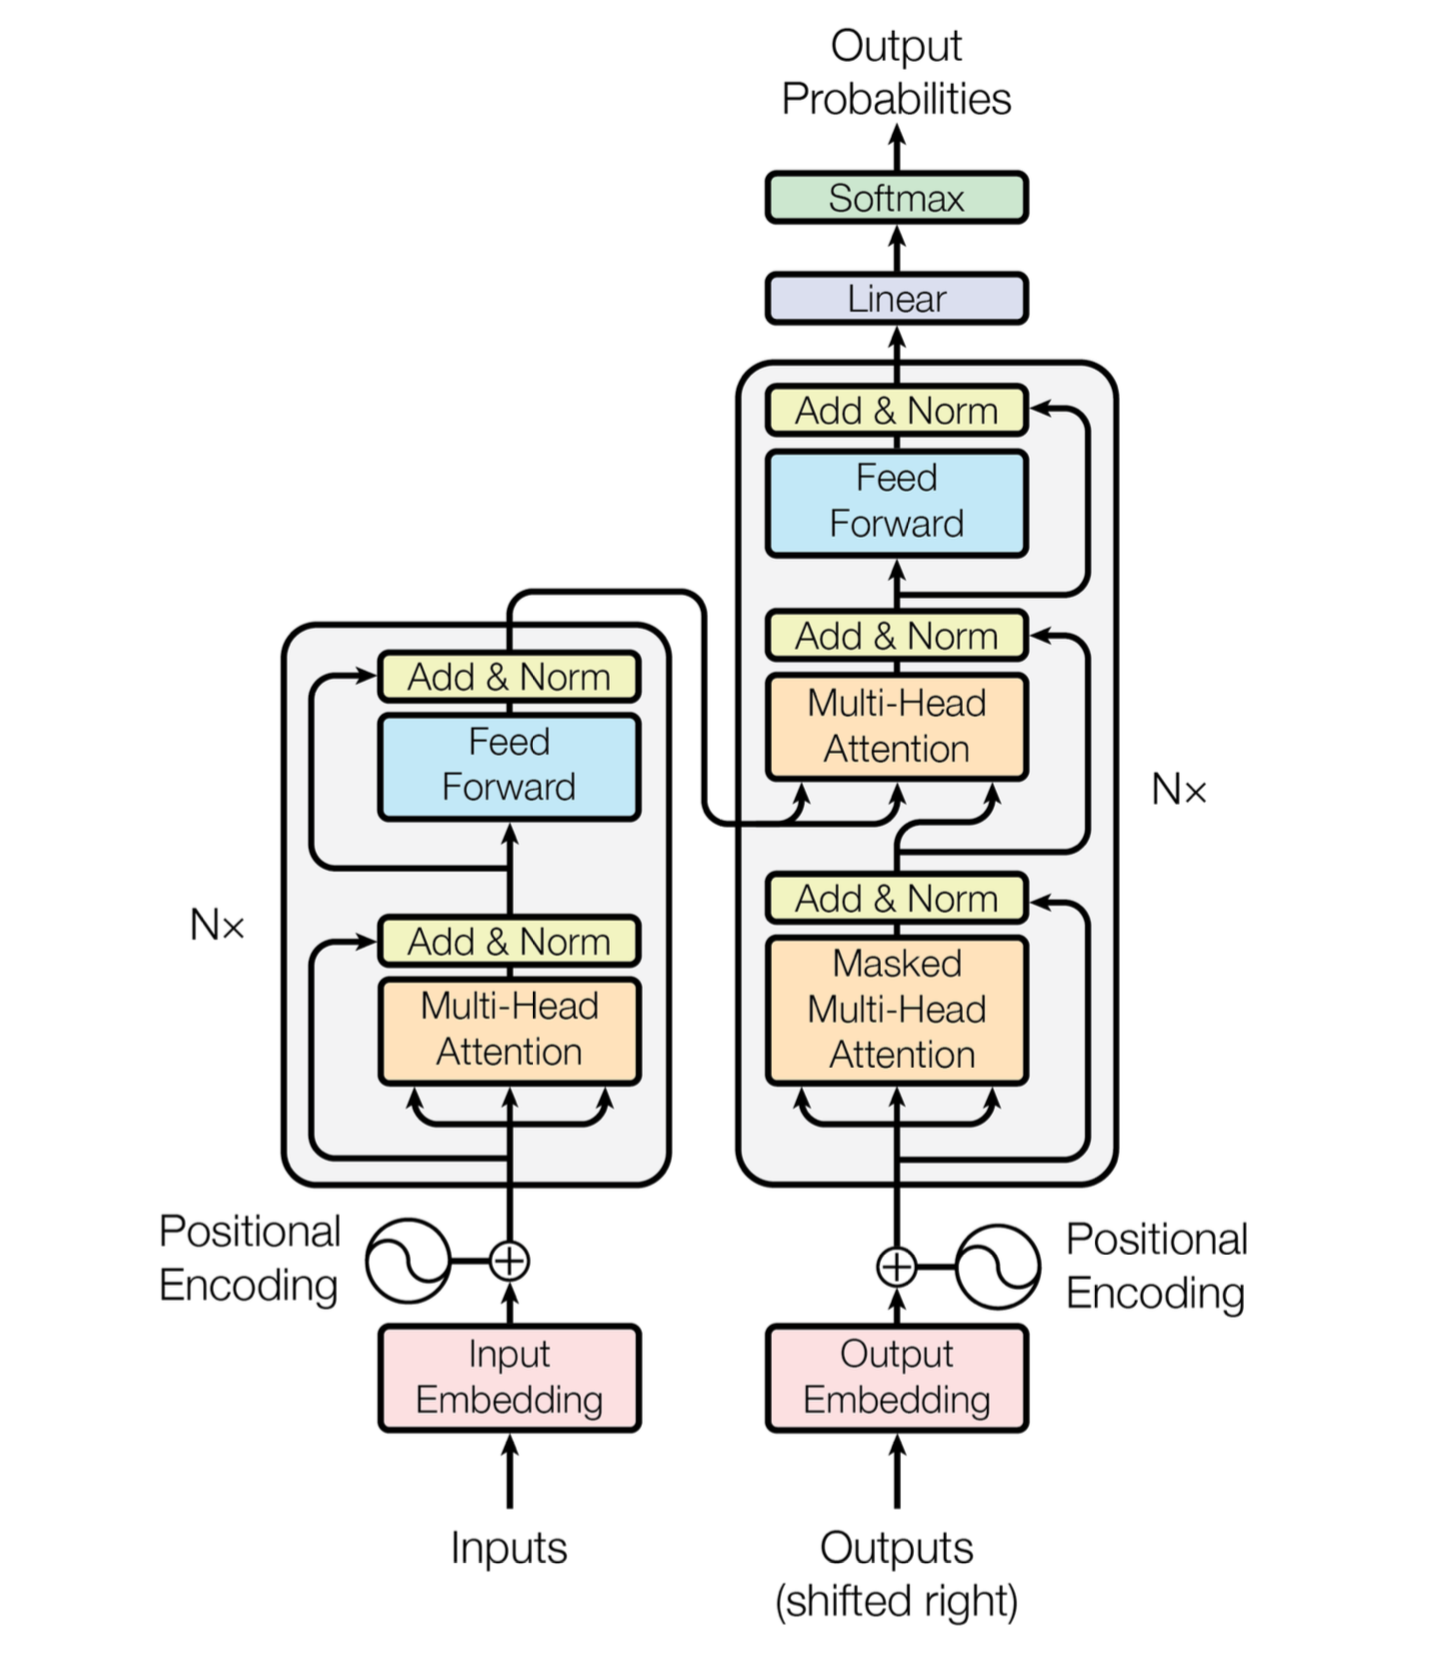
\includegraphics[scale=0.35]{images/transformer/transformer_model_architecture.png}
    \caption{Transformer architecture}
    \label{fig:transformer_architecture}
\end{figure}

Transformers, like most competitive neural sequence transduction, have an encoder-decoder structure with the encoder mapping to an input sequence of symbols $(x_1, \dots, x_n)$ to a continuous representation $z = (z_1, \dots, z_n)$. Given $z$, the decoder generates an output sequence $(y_1, \dots, y_m)$ of symbols one element at a time. In the left and right halves of Figure \ref{fig:transformer_architecture} is shown the fully-connected layers of both encoders and decoders.
\subsection{Encoder}
The encoder is composed of a stack of $N=6$ identical layers, each one has two sub-layers:
\begin{itemize}
    \item a multi-head self-attention mechanism
    \item a position-wise fully connected feed-forward network
\end{itemize}
A residual connection followed by layer normalization is employed around each sub-layer. All sub-layers in the model produce an output of dimension $d_{model} = 512$.

\subsection{Decoder}
The decoder is composed of a stack of $N=6$ identical layers. The decoder inserts a third sub-layer to the two encoder sub-layer. This sub-layer performs multi-head attention over the output of the encoder stack. Similarly to the encoder, around each of the sub-layers are employed residual connections followed by layer normalization. The self-attention sub-layer is modified in the decoder stack to prevent positions from attending to subsequent positions. This kind of masking, combined with fact that the output embeddings are offset by one position, ensures that the predictions for position i can depend only on the known outputs at positions less than i. All sub-layers in the model produce an output of dimension $d_{model} = 512$.

\subsection{Attention}
An attention function consists in mapping a query and a set of key-value pairs to an output, where the query, keys, values and output are all vectors. The output is computed as a weighted sum of the values, with weights computed by a compatibility function of the query with the corresponding key.
\subsubsection{Scaled dot-product attention} 
\begin{figure}[h]
    \centering
    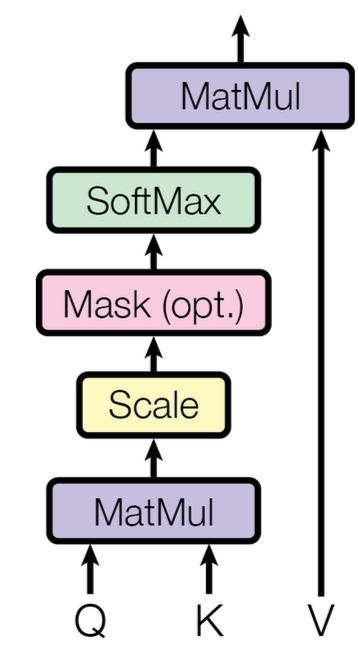
\includegraphics[scale=0.35]{images/transformer/scaled_dot_product_attention.png}
    \caption{Scaled dot-product attention}
    \label{fig:scaled_dot-product_attention}
\end{figure}
The input consists of queries and keys of dimension $d_k$, and values of dimension $d_v$.
To obtain the weights on the values, the dot product of the query with all keys is performed, dividing each by $\sqrt{d_k}$ and applying a softmax function.
The queries, values and keys sets are packed together into Q (queries), K (keys) and V (values) sets. 
The attention function is computed using Q, K and V matrices, producing an output matrix in this way:
\begin{center}
    $Attention(Q, K, V) = softmax(\frac{QK^T}{\sqrt{d_k}})V$
\end{center}
Scaled dot-product attention is both faster and more space efficient of two commonly used attention functions: additive attention and dot-product (multiplicative) attention. These performances reachable because of the highly optimized implementation of matrix multiplication code.
\subsubsection{Multi-head attention}
\begin{figure}[h]
    \centering
    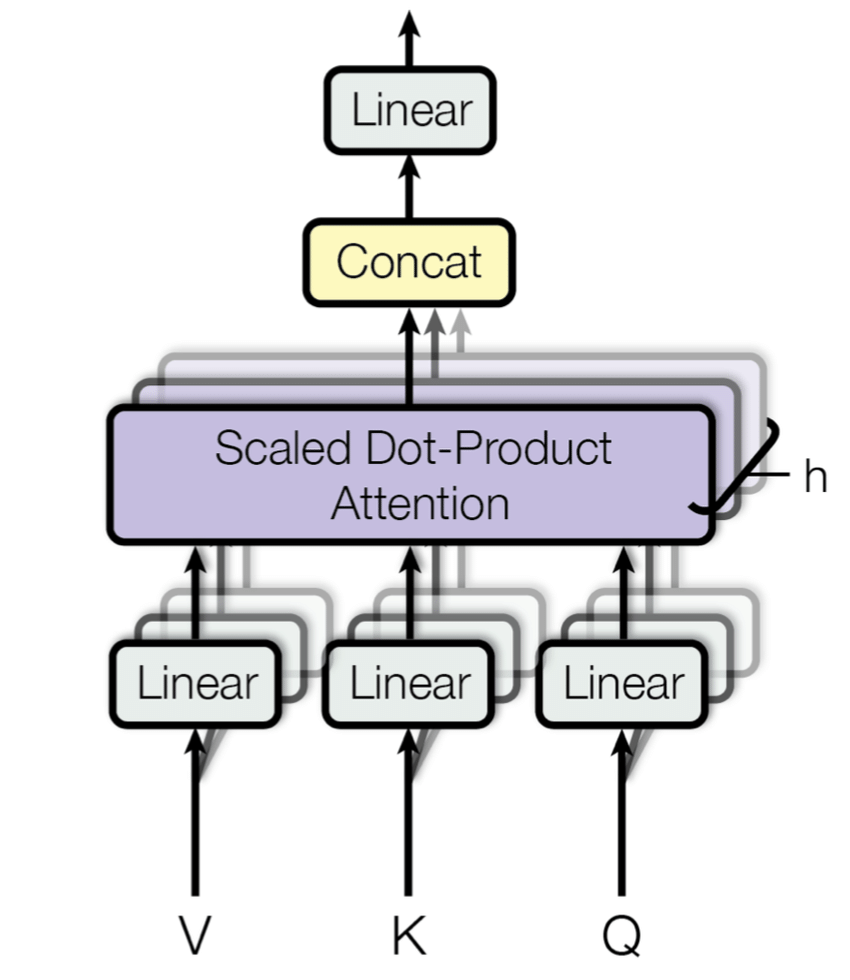
\includegraphics[scale=0.25]{images/transformer/multi-headed_attention.jpeg}
    \caption{Multi-head attention}
    \label{fig:multi-head_attention}
\end{figure}
As visible in Figure \ref{fig:multi-head_attention}, queries, values and keys are linearly projected $h$ times, with different learned linear projections to $d_k$, $d_q$ and $d_v$ dimensions respectively. The attention function is performed in parallel on each projection, yielding $d_v$-dimensional output values. These are concatenated and once again projected, resulting in the final values. \\
Multi-head attention allows the model to jointly attend to information form different representation subspaces at different position. 
\begin{center}
    $MultiHead(Q, V, K) = Concat(head_1, \dots, head_h)W^O$\\
    where $head_i = Attention(QW^Q_i, KW^K_i, VW^V_i)$
\end{center}
Where the projections are parameter matrices $W^Q_i\in\R^{d_{model \times d_k}}, W^K_i\in\R^{d_{model \times d_k}}, W^V_i\in\R^{d_{model \times d_k}}$ and $ W^O_i\in\R^{d_{model \times d_k}}$.

\subsection{Position-wise Feed-Forward Networks}
Every layer in both encoders and decoders contain a fully connected feed-forward neural network, which is applied to each position separately and identically.
It consists of two linear transformations with a ReLU activation in between.
\begin{center}
    $FFN(x) = max(0, xW_1 + b_1)W_2 + b_2$
\end{center}
The linear transformations remain the same across different positions, using different parameters on each layer. The dimensionality of input and output is $d_{model} = 512$, and the inner-layer has dimensionality $d_{ff} = 2048$.

\subsection{Embeddings and softmax}
Learned embeddings are used to convert the input and output tokens to vectors of dimension $d_{model}$. The learned linear transformation and softmax function are used to convert the decoder output to predicted next-token probabilities.

\subsection{Positional encodings}
Since the model contains neither recurrence nor convolution, relative or absolute tokens positional encodings are injected in order to make use of the order of the sequence. Positional encodings are added to the input embeddings of the encoder and decoder stacks. They have the same dimension $d_{model}$ as the embeddings, so the two can be summed.

\subsection{Self-attention motivations}
In order to understand why self-attention layers are used, it's necessary to compare them with recurrent and convolutional layers. There are three aspects that are important to consider: the total computation complexity per layer, the amount of computation that can be parallelized (intended as the minimum number of sequential operations required) and the path length between long-range dependencies in the network. \\
In terms of computation that can be parallelized, a self-attention layer connects all positions with a constant number of sequentially executed operations, whereas a recurrent layer requires $O(n)$ sequential operations. In terms of computational complexity, self-attention layers are faster than recurrent layers when the sequence length n is smaller than the representation dimensionality d, which is most often the case with sentence representations used by state-of-the-art models in machine translations, such as word-piece and byte-pair representations.

\begin{table}[h!]
\centering
\begin{tabular}{||c c c c||} 
 \hline
 Layer type & Complexity per layer & Sequential operations & Maximum path length \\ [0.5ex] 
 \hline\hline
 Self attention & $O(n^2 \cdot d)$ & $O(1)$ & $O(1)$ \\ 
 \hline
 Recurrent & $O(n \cdot d^2)$ & $O(n)$ & $O(n)$ \\
 \hline
 Convolutional & $O(k \cdot n \cdot d^2)$ & $O(1)$ & $O(log_k(n))$ \\
 \hline
 
\end{tabular}
\caption{Self attention complexity}
 \label{table:complexity_self_attention}
\end{table}


\end{document}